% !TeX spellcheck = en_GB
\documentclass[AERbeamer%              style
              ,optEnglish%            language
              %,handout%               deactivate animation
              ,optBiber%               bibliography tool
              ,optBibstyleAlphabetic%
              ,optBeamerClassicFormat% 4:3 format
              %,optBeamerWideFormat%   16:9 format
              ]{AERlatex}%
\setbeameroption{show notes}% Show all notes
%
% Set paths
\graphicspath{{figures_lecture_2/}}%
\addbibresource{literature.bib}%
%
% Package Imports
%\usepackage{media9}
\usepackage{graphicx}
\usepackage{multimedia}
\usepackage{subcaption}
\usepackage{amsmath}
%
% set meta data
\title{Probabilistic Programming for Scientific Discovery}%
\subtitle{Lecture 2}
\author{Ludger Paehler}% (optional)
\date{\AERutilsDate{29}{7}{2020}}% (optional)
\institute{Lviv Data Science Summer School}% (optional)
%
% Setup of header and footer
\AERbeamerSetupHeader{\AERlayoutHeaderCDChair}%
\AERbeamerSetupFooterCD%
%\AERbeamerSetupFooterSlideNumberOnly%
%
\begin{document}%
%
% Start with titlepage
\AERbeamerTitlePageDefault%
%
%\begin{frame}{Title of Slide}{Subtitle of Slide}%
%    \blindtext%
%\end{frame}%
%

% Slide 0: Table of Contents
\begin{frame}{Table of Contents}{}%
    % Contents
    \tableofcontents
\end{frame}%


% Approaches to Inference, the Core of every respectable Probabilistic Programming Framework
\section{Approaches to Inference - the Inference Engines}


% Introductory slide to show how everything centers around the inference algorithm library in probabilistic programming
\begin{frame}[c]{Approaches to Inference - the Inference Engines}
    % Two columns, explanation on the left probabilistic programming system explanation on the right
    \begin{columns}[T]
        % Explaining the typical construction of a PPS
        \begin{column}{0.48\textwidth}
            \centering
            \begin{itemize}
                \item A typical probabilistic programming system consists of:
                \begin{itemize}
                    \item A domain-specific language (DSL), which enables the user to express his model using the language-specific primitives
                    \item Provides a library of inference algorithms, which enable inference on probabilistic models definable in the
                          DSL.
                    \item Prevalent Monte-Carlo and variational inference approaches have their own specific sets of strength, it is
                          hence important to understand the inference algorithms one utilizes
                \end{itemize}
            \end{itemize}
        \end{column}
        % Illustration of a typical PPS
        \begin{column}{0.48\textwidth}
            \centering
            \begin{figure}
                \centering
                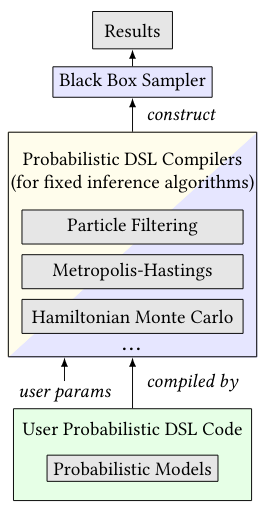
\includegraphics[width=0.4\textwidth]{TypicalPPS.png}
                \caption{Structure of a typical probabilistic programming system. Source: \textit{Gen: A General-Purpose Probabilistic Programming Systems with Programmable Inference}}
            \end{figure}
        \end{column}
    \end{columns}
\end{frame}


% Subsection for Monte-Carlo algorithms of all flavours
\subsection{Monte-Carlo}


\subsubsection*{Hamiltonian Monte Carlo}
% Hamiltonian Monte-Carlo Slide 1
\begin{frame}[c]{Monte-Carlo Approaches to Inference}{Hamiltonian Monte-Carlo \footnote{Neal, R.M., 2011. MCMC using Hamiltonian dynamics. Handbook of markov chain monte carlo, 2(11), p.2.}}
    \centering
    \begin{itemize}
        \item Hamiltonian Monte-Carlo 1
    \end{itemize}
\end{frame}


% Hamiltonian Monte-Carlo Slide 2
\begin{frame}[c]{Monte-Carlo Approaches to Inference}{Hamiltonian Monte-Carlo}
    \centering
    \begin{itemize}
        \item Hamiltonian Monte-Carlo 2
    \end{itemize}
\end{frame}


% Hamiltonian Monte-Carlo Slide 3
\begin{frame}[c]{Monte-Carlo Approaches to Inference}{Hamiltonian Monte-Carlo}
    \centering
    \begin{itemize}
        \item Hamiltonian Monte-Carlo 3
    \end{itemize}
\end{frame}


% Hamiltonian Monte-Carlo Slide 4
\begin{frame}[c]{Monte-Carlo Approaches to Inference}{Hamiltonian Monte-Carlo}
    \centering
    \begin{itemize}
        \item Hamiltonian Monte-Carlo 4
    \end{itemize}
\end{frame}



\subsubsection*{Random-Walk Metropolis Hastings}
% Random-Walk Metropolis Hastings Slide 1
\begin{frame}[c]{Monte-Carlo Approaches to Inference}{Random-Walk Metropolis Hastings \footnote{Gelman, A., Carlin, J.B., Stern, H.S., Dunson, D.B., Vehtari, A. and Rubin,
                                                                                                D.B., 2013. Bayesian data analysis. CRC press.}
                                                                                      \footnote{Gilks, W.R. and Richardson, S., S. and Spiegelhalter, D.(1996). Markov chain
                                                                                                Monte Carlo in practice. London, UK: Chapman k Hall/CRC.}}
    \centering
    \begin{itemize}
        \item Random-Walk Metropolis Hastings 1
    \end{itemize}
\end{frame}


% Random-Walk Metropolis Hastings Slide 2
\begin{frame}[c]{Monte-Carlo Approaches to Inference}{Random-Walk Metropolis Hastings}
    \centering
    \begin{itemize}
        \item Random-Walk Metropolis Hastings 2
    \end{itemize}
\end{frame}


% Random-Walk Metropolis Hastings Slide 3
\begin{frame}[c]{Monte-Carlo Approaches to Inference}{Random-Walk Metropolis Hastings}
    \centering
    \begin{itemize}
        \item Random-Walk Metropolis Hastings 3
    \end{itemize}
\end{frame}


% Random-Walk Metropolis Hastings Slide 4
\begin{frame}[c]{Monte-Carlo Approaches to Inference}{Random-Walk Metropolis Hastings}
    \centering
    \begin{itemize}
        \item Random-Walk Metropolis Hastings 4
    \end{itemize}
\end{frame}



\subsubsection*{Stochastic-Gradient Langevin Dynamics}
% Stochastic-Gradient Langevin Dynamic Monte-Carlo Slide 1
\begin{frame}[c]{Monte-Carlo Approaches to Inference}{Stochastic-Gradient Langevin Dynamics \footnote{Welling, M. and Teh, Y.W., 2011. Bayesian learning via stochastic gradient Langevin
                                                                                                      dynamics. In Proceedings of the 28th international conference on machine learning
                                                                                                      (ICML-11) (pp. 681-688).}
                                                                                            \footnote{Brosse, N., Durmus, A. and Moulines, E., 2018. The promises and pitfalls of stochastic
                                                                                                      gradient Langevin dynamics. In Advances in Neural Information Processing Systems (pp. 8268-8278).}}
    \centering
    \begin{itemize}
        \item Stochastic-Gradient Langevin Dynamics 1
    \end{itemize}
\end{frame}


% Stochastic-Gradient Langevin Dynamic Monte-Carlo Slide 2
\begin{frame}[c]{Monte-Carlo Approaches to Inference}{Stochastic-Gradient Langevin Dynamics}
    \centering
    \begin{itemize}
        \item Stochastic-Gradient Langevin Dynamics 2
    \end{itemize}
\end{frame}


% Stochastic-Gradient Langevin Dynamic Monte-Carlo Slide 3
\begin{frame}[c]{Monte-Carlo Approaches to Inference}{Stochastic-Gradient Langevin Dynamics}
    \centering
    \begin{itemize}
        \item Stochastic-Gradient Langevin Dynamics 3
    \end{itemize}
\end{frame}


% Stochastic-Gradient Langevin Dynamic Monte-Carlo Slide 4
\begin{frame}[c]{Monte-Carlo Approaches to Inference}{Stochastic-Gradient Langevin Dynamics}
    \centering
    \begin{itemize}
        \item Stochastic-Gradient Langevin Dynamics 4
    \end{itemize}
\end{frame}



% Variational Inference
\subsection{Variational Inference}

\subsubsection*{Classical Variational Inference}
% Variational Inference Slide 1
\begin{frame}[c]{Variational Approaches to Inference}{Variational Inference \footnote{Blei, D.M., Kucukelbir, A. and McAuliffe, J.D., 2017. Variational inference: A
                                                                                      review for statisticians. Journal of the American statistical Association, 112(518),
                                                                                      pp.859-877.}
                                                                            \footnote{Zhang, C., Bütepage, J., Kjellström, H. and Mandt, S., 2018. Advances in variational inference.
                                                                                      IEEE transactions on pattern analysis and machine intelligence, 41(8), pp.2008-2026.}}
    \centering
    \begin{itemize}
        \item Variational Inference 1
    \end{itemize}
\end{frame}


% Variational Inference Slide 2
\begin{frame}[c]{Variational Approaches to Inference}{Variational Inference}
    \centering
    \begin{itemize}
        \item Variational Inference 2
    \end{itemize}
\end{frame}


% Variational Inference Slide 3
\begin{frame}[c]{Variational Approaches to Inference}{Variational Inference}
    \centering
    \begin{itemize}
        \item Variational Inference 3
    \end{itemize}
\end{frame}


% Variational Inference Slide 4
\begin{frame}[c]{Variational Approaches to Inference}{Variational Inference}
    \centering
    \begin{itemize}
        \item Variational Inference 4
    \end{itemize}
\end{frame}



\subsubsection*{Stochastic Variational Inference}
% Stochastic Variational Inference Slide 1
\begin{frame}[c]{Variational Approaches to Inference}{Stochastic Variational Inference \footnote{Hoffman, M.D., Blei, D.M., Wang, C. and Paisley, J., 2013. Stochastic variational
                                                                                                 inference. The Journal of Machine Learning Research, 14(1), pp.1303-1347.}
                                                                                       \footnote{Robbins, H. and Monro, S., 1951. A stochastic approximation method. The annals of 
                                                                                                 mathematical statistics, pp.400-407.}}
    \centering
    \begin{itemize}
        \item Stochastic Variational Inference 1
    \end{itemize}
\end{frame}


% Stochastic Variational Inference Slide 2
\begin{frame}[c]{Variational Approaches to Inference}{Stochastic Variational Inference}
    \centering
    \begin{itemize}
        \item Stochastic Variational Inference 2
    \end{itemize}
\end{frame}


% Stochastic Variational Inference Slide 3
\begin{frame}[c]{Variational Approaches to Inference}{Stochastic Variational Inference}
    \centering
    \begin{itemize}
        \item Stochastic Variational Inference 3
    \end{itemize}
\end{frame}


% Stochastic Variational Inference Slide 4
\begin{frame}[c]{Variational Approaches to Inference}{Stochastic Variational Inference}
    \centering
    \begin{itemize}
        \item Stochastic Variational Inference 4
    \end{itemize}
\end{frame}



\subsubsection*{Automatic Differentiation Variational Inference}
% Automatic Differentiation Variational Inference Slide 1
\begin{frame}[c]{Variational Approaches to Inference}{Automatic Differentiation Variational Inference \footnote{Kucukelbir, A., Tran, D., Ranganath, R., Gelman, A. and Blei, D.M., 2017.
                                                                                                                Automatic differentiation variational inference. The Journal of Machine
                                                                                                                Learning Research, 18(1), pp.430-474.}
                                                                                                      \footnote{Kucukelbir, A., Ranganath, R., Gelman, A. and Blei, D., 2015. Automatic
                                                                                                                variational inference in Stan. In Advances in neural information processing
                                                                                                                systems (pp. 568-576).}}
    \centering
    \begin{itemize}
        \item Automatic Differentiation Variational Inference 1
    \end{itemize}
\end{frame}


% Automatic Differentiation Variational Inference Slide 2
\begin{frame}[c]{Variational Approaches to Inference}{Automatic Differentiation Variational Inference}
    \centering
    \begin{itemize}
        \item Automatic Differentiation Variational Inference 2
    \end{itemize}
\end{frame}


% Automatic Differentiation Variational Inference Slide 3
\begin{frame}[c]{Variational Approaches to Inference}{Automatic Differentiation Variational Inference}
    \centering
    \begin{itemize}
        \item Automatic Differentiation Variational Inference 3
    \end{itemize}
\end{frame}


% Automatic Differentiation Variational Inference Slide 4
\begin{frame}[c]{Variational Approaches to Inference}{Automatic Differentiation Variational Inference}
    \centering
    \begin{itemize}
        \item Automatic Differentiation Variational Inference 4
    \end{itemize}
\end{frame}



\subsubsection*{Black-Box Variational Inference}
% Black-Box Variational Inference Slide 1
\begin{frame}[c]{Variational Approaches to Inference}{Black Box Variational Inference \footnote{Ranganath, R., Gerrish, S. and Blei, D., 2014, April. Black box
                                                                                                variational inference. In Artificial Intelligence and Statistics (pp. 814-822).}
                                                                                      \footnote{Chu, C., Minami, K. and Fukumizu, K., 2020. The equivalence between Stein
                                                                                                variational gradient descent and black-box variational inference. arXiv preprint arXiv:2004.01822.}}
    \centering
    \begin{itemize}
        \item Black Box Variational Inference 1
    \end{itemize}
\end{frame}


% Black-Box Variational Inference Slide 2
\begin{frame}[c]{Variational Approaches to Inference}{Black Box Variational Inference}
    \centering
    \begin{itemize}
        \item Black Box Variational Inference 2
    \end{itemize}
\end{frame}


% Black-Box Variational Inference Slide 3
\begin{frame}[c]{Variational Approaches to Inference}{Black Box Variational Inference}
    \centering
    \begin{itemize}
        \item Black Box Variational Inference 3
    \end{itemize}
\end{frame}


% Black-Box Variational Inference Slide 4
\begin{frame}[c]{Variational Approaches to Inference}{Black Box Variational Inference}
    \centering
    \begin{itemize}
        \item Black Box Variational Inference 4
    \end{itemize}
\end{frame}




% Probabilistic Programming Frameworks
\section{Probabilistic Programming Frameworks}


\subsection{Stan}
% Stan Slide 1: general introduction
\begin{frame}[c]{Stan \footnote{Carpenter, B., Gelman, A., Hoffman, M.D., Lee, D.,
                                Goodrich, B., Betancourt, M., Brubaker, M., Guo, J., Li, P.
                                and Riddell, A., 2017. Stan: A probabilistic programming
                                language. Journal of statistical software, 76(1).}}{Overview}
    \centering
    \begin{itemize}
        \item General overview of the purpose behind Stan
    \end{itemize}
\end{frame}


% Stan Slide 2: Example Code
\begin{frame}[c]{Stan}{Syntax}
    \centering
    \begin{itemize}
        \item Example code to get a grasp for the syntax
    \end{itemize}
\end{frame}


% Stan Slide 3: Application Performance
\begin{frame}[c]{Stan}{Application Performance}
    \centering
    \begin{itemize}
        \item Example applications
    \end{itemize}
\end{frame}


\subsection{Venture}
% Venture (2014) Slide 1: General Introduction
\begin{frame}[c]{Venture \footnote{Mansinghka, V., Selsam, D. and Perov, Y., 2014.
                                   Venture: a higher-order probabilistic programming platform
                                   with programmable inference. arXiv preprint arXiv:1404.0099.}
                         \footnote{Goodman, N., Mansinghka, V., Roy, D.M., Bonawitz, K. and Tenenbaum, J.B., 2012.
                                   Church: a language for generative models. arXiv preprint arXiv:1206.3255.}}{Overview}
    \centering
    \begin{itemize}
        \item General overview of the purpose behind venture
    \end{itemize}
\end{frame}


% Venture Slide 2: Example Code
\begin{frame}[c]{Venture}{Syntax}
    \centering
    \begin{itemize}
        \item Example code to get a gauge for the syntax
    \end{itemize}
\end{frame}


% Venture Slide 3: Application Performance
\begin{frame}[c]{Venture}{Application Performance}
    \centering
    \begin{itemize}
        \item Application performance
    \end{itemize}
\end{frame}


\subsection{Anglican}
% Anglican (2014): General Introduction
\begin{frame}[c]{Anglican \footnote{Tolpin, D., van de Meent, J.W., Yang, H. and Wood, F., 2016, August. Design
                                    and implementation of probabilistic programming language anglican. In Proceedings
                                    of the 28th Symposium on the Implementation and Application of Functional
                                    programming Languages (pp. 1-12).}}{Overview}
    \centering
    \begin{itemize}
        \item General overview of the purpose behind Anglican
    \end{itemize}
\end{frame}


% Anglican Slide 2: Example Code
\begin{frame}[c]{Anglican}{Syntax}
    \centering
    \begin{itemize}
        \item Example code
    \end{itemize}
\end{frame}


% Anglican Slide 3: Application Performance
\begin{frame}[c]{Anglican}{Application Performance}
    \centering
    \begin{itemize}
        \item Application performance
    \end{itemize}
\end{frame}


\subsection{PyMC3}
% PyMC3 (2015) Slide 1: General Introdction
\begin{frame}[c]{PyMC3 \footnote{Salvatier, J., Wiecki, T.V. and Fonnesbeck, C., 2016. Probabilistic programming
                                 in Python using PyMC3. PeerJ Computer Science, 2, p.e55.}}{Overview}
    \centering
    \begin{itemize}
        \item General overview of the purpose behind PcMC3
    \end{itemize}
\end{frame}


% PyMC3 Slide 2: Example Code
\begin{frame}[c]{PyMC3}{Syntax}
    \centering
    \begin{itemize}
        \item Example code
    \end{itemize}
\end{frame}


% PyMC3 Slide 3: Application Performance
\begin{frame}[c]{PyMC3}{Application Performance}
    \centering
    \begin{itemize}
        \item Application performance
    \end{itemize}
\end{frame}


\subsection{TensorFlow Probability}
% TensorFlow Probability (2017) Slide 1: General Introduction
\begin{frame}[c]{TensorFlow Probability \footnote{Dillon, J.V., Langmore, I., Tran, D., Brevdo, E., Vasudevan, S.,
                                                  Moore, D., Patton, B., Alemi, A., Hoffman, M. and Saurous, R.A., 2017.
                                                  Tensorflow distributions. arXiv preprint arXiv:1711.10604.}}{Overview}
    \centering
    \begin{itemize}
        \item General overview of the purpose behind Tensorflow Probability
    \end{itemize}
\end{frame}


% Tensorflow Probability Slide 2: Example Code
\begin{frame}[c]{TensorFlow Probability}{Syntax}
    \centering
    \begin{itemize}
        \item Example code
    \end{itemize}
\end{frame}


% Tensorflow Probability Slide 3: Application Performance
\begin{frame}[c]{TensorFlow Probability}{Application Performance}
    \centering
    \begin{itemize}
        \item Application performance
    \end{itemize}
\end{frame}


\subsection{Pyro \& NumPyro}
% Pyro (2018) Slide 1: General introduction
\begin{frame}[c]{Pyro \footnote{Bingham, E., Chen, J.P., Jankowiak, M., Obermeyer, F., Pradhan, N., Karaletsos, T.,
                                Singh, R., Szerlip, P., Horsfall, P. and Goodman, N.D., 2019. Pyro: Deep universal
                                probabilistic programming. The Journal of Machine Learning Research, 20(1), pp.973-978.}
                \& NumPyro \footnote{Phan, D., Pradhan, N. and Jankowiak, M., 2019. Composable effects for flexible and
                                     accelerated probabilistic programming in NumPyro. arXiv preprint arXiv:1912.11554.}}{Overview}
    \centering
    \begin{itemize}
        \item General overview of the purpose behind Pyro \& NumPyro
    \end{itemize}
\end{frame}


% Pyro & NumPyro Slide 2: Example Code
\begin{frame}[c]{Pyro \& NumPyro}{Syntax}
    \centering
    \begin{itemize}
        \item Example code of Pyro \& NumPyro
    \end{itemize}
\end{frame}


% Pyro & NumPyro Slide 3: Application Performance  -> Might want to add a second slide here for the performance of NumPyro
\begin{frame}[c]{Pyro \& NumPyro}{Application Performance}
    \centering
    \begin{itemize}
        \item Application performance
    \end{itemize}
\end{frame}


\subsection{Edward2}
% Edward2 (2018/2019) Slide 1: General introduction
\begin{frame}[c]{Edward2 \footnote{Tran, D., Hoffman, M.W., Moore, D., Suter, C., Vasudevan, S. and Radul, A., 2018. Simple, distributed,
                                   and accelerated probabilistic programming. In Advances in Neural Information Processing Systems (pp. 7598-7609).}
                         \footnote{Tran, D., Dusenberry, M., van der Wilk, M. and Hafner, D., 2019. Bayesian layers: A module for neural network
                                   uncertainty. In Advances in Neural Information Processing Systems (pp. 14660-14672).}}{Overview}
    \centering
    \begin{itemize}
        \item General overview of the purpose behind Edward2
    \end{itemize}
\end{frame}


% Edward2 Slide 2: Example Code
\begin{frame}[c]{Edward2}{Syntax}
    \centering
    \begin{itemize}
        \item Example code of Edward2
    \end{itemize}
\end{frame}


% Edward2 Slide 3: Application Performance
\begin{frame}[c]{Edward2}{Application Performance}
    \centering
    \begin{itemize}
        \item Application performance
    \end{itemize}
\end{frame}


\subsection{Gen}
% Gen (2019) Slide 1: General introduction
\begin{frame}[c]{Gen \footnote{Cusumano-Towner, M.F., Saad, F.A., Lew, A.K. and Mansinghka, V.K., 2019, June. Gen: a general-purpose
                               probabilistic programming system with programmable inference. In Proceedings of the 40th ACM SIGPLAN
                               Conference on Programming Language Design and Implementation (pp. 221-236).}
                     \footnote{Cusumano-Towner, M., Lew, A.K. and Mansinghka, V.K., 2020. Automating Involutive MCMC using
                               Probabilistic and Differentiable Programming. arXiv preprint arXiv:2007.09871.}}{Overview}
    \centering
    \begin{itemize} % Mention the programmable inference to push the boundaries of prob prog here
        \item General overview of the purpose behind Gen
    \end{itemize}
\end{frame}


% Gen Slide 2: Difference to other probabilistic programming system
\begin{frame}[c]{Gen}{Programmable Inference}
    \centering
    \begin{itemize}
        \item Illustration of Gen's slightly different construction compared to the other frameworks
    \end{itemize}
\end{frame}

% Gen Slide 3: Example Code
\begin{frame}[c]{Gen}{Syntax}
    \centering
    \begin{itemize}
        \item Example code of Gen
    \end{itemize}
\end{frame}


% Gen Slide 4: Application perforance
\begin{frame}[c]{Gen}{Application Performance}
    \centering
    \begin{itemize}
        \item Application performance
    \end{itemize}
\end{frame}


\subsection{PyProb}
% PyProb (2019) Slide 1: General introduction
\begin{frame}[c]{PyProb \footnote{Baydin, A.G., Shao, L., Bhimji, W., Heinrich, L., Naderiparizi, S., Munk, A., Liu, J., Gram-Hansen, B.,
                                  Louppe, G., Meadows, L. and Torr, P., 2019. Efficient probabilistic inference in the quest for physics
                                  beyond the standard model. In Advances in neural information processing systems (pp. 5459-5472).}}{Overview}
    \centering
    \begin{itemize}
        \item General overview of the purpose behind PyProb
    \end{itemize}
\end{frame}


% PyProb Slide 2: Example Code
\begin{frame}[c]{PyProb}{Syntax}
    \centering
    \begin{itemize}
        \item Example code of PyProb
    \end{itemize}
\end{frame}


% PyProb Slide 3: Application performance
\begin{frame}[c]{PyProb}{Application Performance}
    \centering
    \begin{itemize}
        \item Application performance
    \end{itemize}
\end{frame}


\subsection{Turing}
% Turing (2018) Side 1: General introduction
\begin{frame}[c]{Turing \footnote{Ge, H., Xu, K. and Ghahramani, Z., 2018, March. Turing: A Language for Flexible
                                  Probabilistic Inference. In International Conference on Artificial Intelligence
                                  and Statistics (pp. 1682-1690).}}{Overview}
    \centering
    \begin{itemize}
        \item General overview of the purpose behind Turing
    \end{itemize}
\end{frame}


% Turing Slide 2: Example code
\begin{frame}[c]{Turing}{Syntax}
    \centering
    \begin{itemize}
        \item Example code of Turing
    \end{itemize}
\end{frame}


% Turing Slide 3: Application performance
\begin{frame}[c]{Application performance}
    \centering
    \begin{itemize}
        \item Application performance
    \end{itemize}
\end{frame}


% Summary in matrix form
\begin{frame}[c]{Probabilistic Programming Frameworks}{Summary}
    \centering
    \begin{itemize}
        \item Summary of all probabilistic programming frameworks in a single table
    \end{itemize}
\end{frame}



% Practical Introduction to Turing
\section{Practical Introduction to a Probabilistic Programming Framework}


% Slide leading over to the Jupyter notebook
\begin{frame}[c]{Introduction to Turing}
    \centering
    \begin{itemize}
        \item We will do our first steps in a probabilistic programming framework with Turing covering
        \begin{itemize}
            \item The modelling syntax
            \item Sampling
            \item Accessing the trace
            \item Automatic differentiation
            \item Working with dynamic Hamiltonian Monte-Carlo
        \end{itemize}
        \item All content can be accessed in the Jupyter notebook \textbf{IntrotoTuring.ipynb}
    \end{itemize}
\end{frame}


% Extension to a more complex example
\section{Extending the ideas to a more complex examples}


% Slide leading over to the Jupyter notebook
\begin{frame}[c]{More Complex Example in Turing}{Model-based inference for causal effects in completely randomized experiments}
    \centering
    \begin{itemize}
        \item Expanding on the simple syntax we will now move to a more complex case:
        \begin{itemize}
            \item Starting with a Bayesian perspective on causal inference
            \item Assignment mechanisms
            \item Posterior inference
        \end{itemize}
        \item All content can be accessed in the Jupyter notebook \textbf{MBInferenceforCausalEffects.ipynb}
    \end{itemize}
\end{frame}






%
%\AERbeamerSetFooterText{References}%
%\begin{frame}[allowframebreaks]{References}%
%    \printbibliography[heading=none]%
%\end{frame}%
%
% End with titlepage
%\AERbeamerTitlePageDefault%
%
%
\end{document}%
%
%
